\documentclass[a4paper,12pt]{article}
\usepackage[utf8]{inputenc}
\usepackage[spanish]{babel}
\usepackage{color}
\usepackage{parskip}
\usepackage{graphicx}
\usepackage{multirow}
\usepackage{listings}
\usepackage{vmargin}
\graphicspath{ {imagenes/} }
\definecolor{mygreen}{rgb}{0,0.6,0}
\definecolor{lbcolor}{rgb}{0.9,0.9,0.9}
\usepackage{epstopdf}


\setpapersize{A4}
\setmargins{2.5cm}       % margen izquierdo
{1.5cm}                        % margen superior
{16.5cm}                      % anchura del texto
{23.42cm}                    % altura del texto
{10pt}                           % altura de los encabezados
{1cm}                           % espacio entre el texto y los encabezados
{0pt}                             % altura del pie de página
{2cm}     

\lstset{
backgroundcolor=\color{lbcolor},
    tabsize=4,    
%   rulecolor=,
    language=[GNU]C++,
        basicstyle=\tiny,
        aboveskip={1.5\baselineskip},
        columns=fixed,
        showstringspaces=false,
        extendedchars=false,
        breaklines=true,
        prebreak = \raisebox{0ex}[0ex][0ex]{\ensuremath{\hookleftarrow}},
        frame=single,
        showtabs=false,
        showspaces=false,
        showstringspaces=false,
        identifierstyle=\ttfamily,
        keywordstyle=\color[rgb]{0,0,1},
        commentstyle=\color[rgb]{0.026,0.112,0.095},
        stringstyle=\color{red},
        numberstyle=\color[rgb]{0.205, 0.142, 0.73},
%        \lstdefinestyle{C++}{language=C++,style=numbers}’.
}

\begin{document}
\begin{Large}
 NOMBRE: CHRISTOFER FABIÁN CHÁVEZ CARAZAS
\end{Large}

\section{Ejercicio 1}

Dado el siguiente código. Derivar los Casos de Prueba.

\begin{lstlisting}
public void howComplex() {
  int i=20;
  while (i<10) {
    System.out.printf("i is %d", i);
    if (i%2 == 0) {
      System.out.println("even");
    } else {
      System.out.println("odd");
    }
  }
}
\end{lstlisting}

\subsection{Nodos en el código y Grafo}

\begin{lstlisting}
public void howComplex() {
  int i=20;
  '1' while (i<10) {
    System.out.printf("i is %d", i);
    '2' if (i%2 == 0) {
      '3' System.out.println("even");
    '4' } else {
      System.out.println("odd");
    '5' }
  '6' }
'7' } 
\end{lstlisting}

\begin{figure}[h]
 \centering
 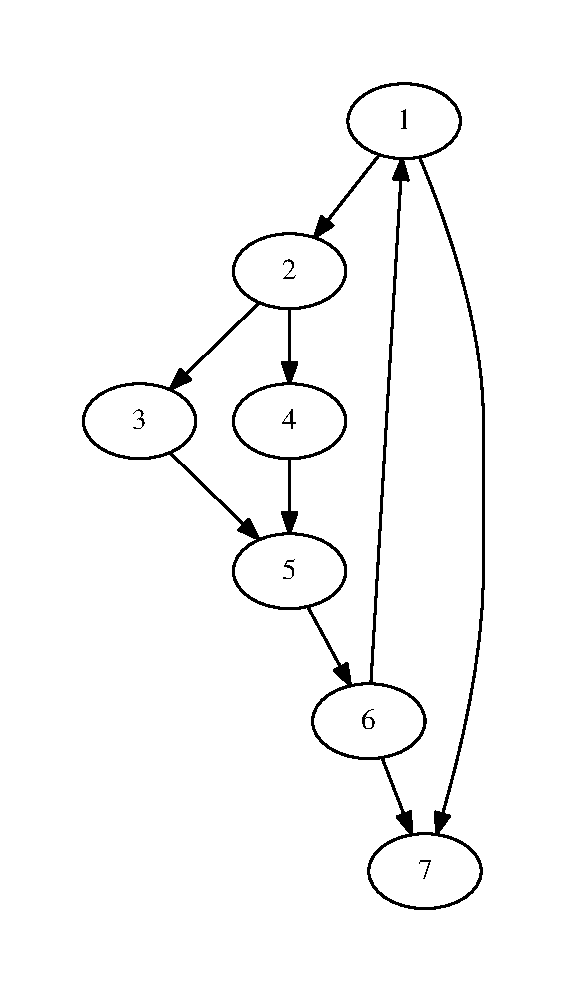
\includegraphics[scale = 0.59]{graf1.pdf}
\end{figure}

\subsection{Complejidad Ciclomática}

\begin{itemize}
 \item V(G) = Número de Regiones = 4;
 \item V(G) = A - N + 2 = 9 - 7 + 2 = 4;
\end{itemize}

\textbf{Caminos:}

\begin{itemize}
 \item Camino 1: 1,7
 \item Camino 2: 1,2,3,5,6,7
 \item Camino 3: 1,2,4,5,6,7
 \item Camino 4: 1,2,3,5,6,1,7
\end{itemize}

\subsection{Casos de Prueba}

\textbf{Caso de Prueba del camino 1:} \\
Entradas: \\
\hspace*{1cm} Un $i$ menor igual a 10 \\
Resultados Esperados: \\
\hspace*{1cm} Finaliza el Programa \par

\textbf{Caso de Prueba del camino 2:} \\
Entradas: \\
\hspace*{1cm} Un $i$ par \\
Resultados Esperados: \\
\hspace*{1cm} Imprime el valor de $i$ \\
\hspace*{1cm} Imprime ``even''  \par

\textbf{Caso de Prueba del camino 3:} \\
Entradas: \\
\hspace*{1cm} Un $i$ impar \\
Resultados Esperados: \\
\hspace*{1cm} Imprime el valor de $i$ \\
\hspace*{1cm} Imprime ``odd'' \par

\textbf{Caso de Prueba del camino 4:} \\
Entradas: \\
\hspace*{1cm} Un $i$ par \\
Resultados Esperados:  \\
\hspace*{1cm} Imprime el valor de $i$ \\
\hspace*{1cm} Imprime ``even'' \\
\hspace*{1cm} Imprime el valor de $i$ \\
\hspace*{1cm} Imprime ``even'' \par

\section{Ejercicio 2}

\begin{lstlisting}
i = 0;
total.entrada = total.valido = 0;
suma = 0;
DO WHILE valor[i] <> -999 and total.entrada < 100
  increment total.entrada in 1;
  IF valor[i] >= minimo AND valor[i] <= maximo
    THEN increment total.valido in 1;
      suma = suma + valor[i];
    ELSE ignore
  ENDIF
  increment i in 1;
ENDDO
IF total.valido > 0
  11 THEN media = suma / total.valido;
  12 ELSE media = -999;
ENDIF
END Media
\end{lstlisting}

\subsection{Nodos en el código y Grafo}

\begin{lstlisting}
i = 0;
total.entrada = total.valido = 0;
suma = 0;
'1' DO WHILE valor[i] <> -999 and total.entrada < 100
  increment total.entrada in 1;
  '2' IF valor[i] >= minimo AND valor[i] <= maximo
    '3' THEN increment total.valido in 1;
      suma = suma + valor[i];
    '4' ELSE ignore
  '5' ENDIF
  increment i in 1;
'6' ENDDO
'7' IF total.valido > 0
  '8' THEN media = suma / total.valido;
  '9' ELSE media = -999;
'10' ENDIF
'11' END Media 
\end{lstlisting}

\begin{figure}
 \centering
 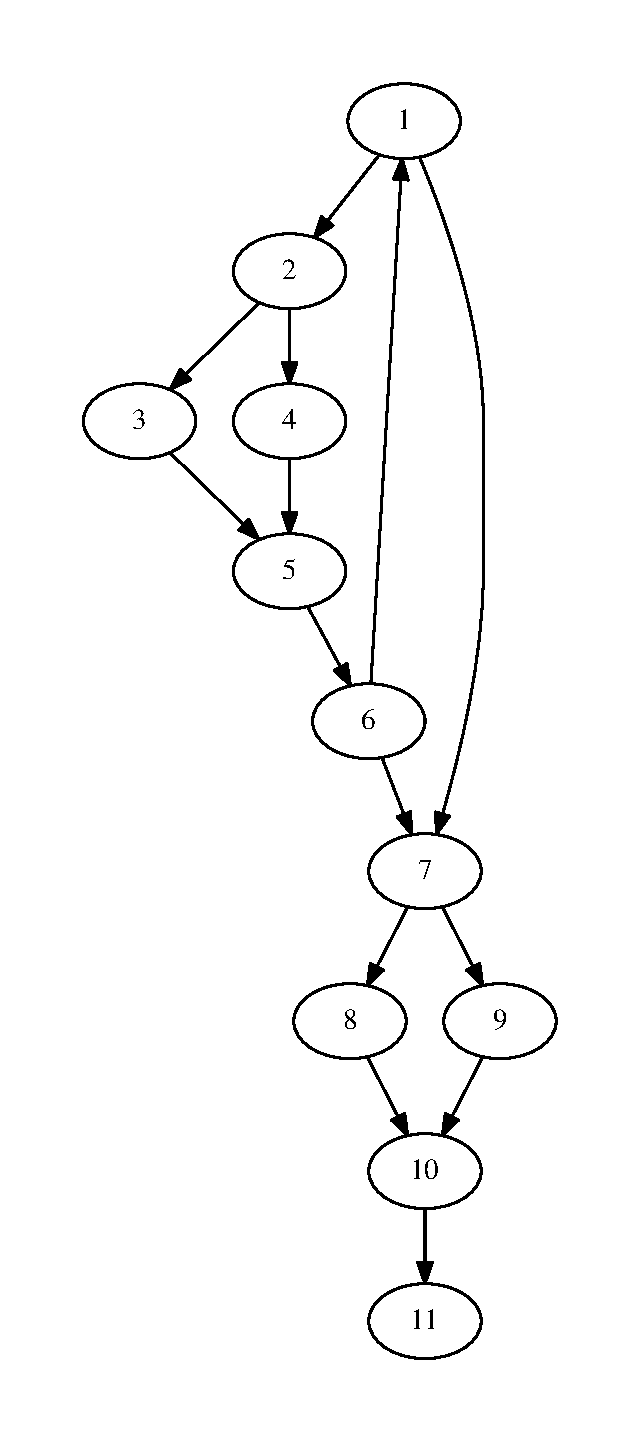
\includegraphics[scale = 1]{graf2.pdf}
\end{figure}

\subsection{Complejidad Ciclomática}

\begin{itemize}
 \item V(G) = Número de Regiones = 5
 \item V(G) = A - N + 2 = 14 - 11 + 2 = 5
\end{itemize}
\textbf{Caminos:}

\begin{itemize}
 \item Camino 1: 1,7,9,10,11
 \item Camino 2: 1,2,3,5,6,7,8,10,11
 \item Camino 3: 1,2,4,5,6,7,9,10,11
 \item Camino 4: 1,2,3,5,6,1,2,3,5,6,7,8,10,11
 \item Camino 5: 1,2,4,5,6,1,2,4,5,6,7,9,10,11
\end{itemize}

\subsection{Casos de Prueba}

\textbf{Caso de Prueba para el camino 1:} \\
Entradas: \\
\hspace*{1cm} El primer número es -999 \\
Resultados Esperados: \\
\hspace*{1cm} Retorna -999 como el valor de la media \\
\hspace*{1cm} El total de entradas es 0 \\
\hspace*{1cm} El total de válidos es 0 \par

\textbf{Caso de Prueba para el camino 2:} \\
Entradas: \\
\hspace*{1cm} Hay un solo valor que esta dentro del rango \\
\hspace*{1cm} El segundo valor es -999 \\
Resultados Esperados: \\
\hspace*{1cm} Retorna el mismo valor como media \\
\hspace*{1cm} El total de entradas es 1 \\
\hspace*{1cm} El total de válidos es 1 \par

\textbf{Caso de Prueba para el camino 3:} \\
Entrada: \\
\hspace*{1cm} Hay un solo valor que no esta dentro del rango \\
\hspace*{1cm} El segundo valor es -999 \\
Resultados Esperados: \\
\hspace*{1cm} Retorna -999 como el valor de la media \\
\hspace*{1cm} El todal de entradas es 1 \\
\hspace*{1cm} El total de válidos es 0 \par

\textbf{Caso de Prueba para el camino 4:} \\
Entradas: \\
\hspace*{1cm} Hay dos valores que están dentro del rango \\
\hspace*{1cm} El tercer valor es -999 \\
Resultados Esperados: \\
\hspace*{1cm} Retorna la suma de los dos valores entre dos como el valor de la media \\
\hspace*{1cm} El total de entradas es 2 \\
\hspace*{1cm} El total de válidos es 2 \par

\textbf{Caso de Prueba para el camino 5:} \\
Entradas: \\
\hspace*{1cm} Hay dos valores que no están dentro del rango \\
\hspace*{1cm} El tercer valor es -999 \\
Resultados Esperados: \\
\hspace*{1cm} Retorna -999 como valor de la media \\
\hspace*{1cm} El total de entradas es 2 \\
\hspace*{1cm} El total de válidos es 0 \par


\end{document}
